\documentclass[11pt,a4paper]{article}
\usepackage[utf8]{inputenc}
\usepackage[T1]{fontenc}
\usepackage[brazil]{babel}
\usepackage{amsmath,booktabs,graphicx,geometry}
\usepackage[authoryear,round]{natbib}
\usepackage{hyperref}
\geometry{margin=2.5cm}
\hypersetup{colorlinks=true,linkcolor=blue,urlcolor=blue,citecolor=blue}

\title{Ganhar a vaga, aparecer no posto:\\
efeitos locais da alocação no Programa Mais Médicos Especialistas sobre adesão,
presença e oferta cadastrada}
\author{Versão curta de trabalho}
\date{16 de setembro de 2026}

\begin{document}
\maketitle

\begin{abstract}
Este artigo curto organiza a evidência empírica do projeto sobre o Programa Mais
Médicos Especialistas (PMM-E) em três camadas com estatutos distintos. A camada
causal explora o limite de seleção de cada vaga: dentro do mesmo curso,
estabelecimento, chamada e modalidade de ampla concorrência, compara o último
candidato selecionado e o primeiro não selecionado quando as pontuações diferem
em exatamente um ponto. Em 36 pares de 2025, ganhar a vaga elevou a homologação
no mesmo curso--CNES em 63,9 pontos percentuais e a presença ativa nesse mesmo
curso--CNES, em 12 de agosto de 2026, em 33,3 pontos percentuais; o placebo
imediatamente abaixo do cutoff é nulo, janelas de gap e exclusões sucessivas
preservam o resultado, e 11 pares de 2026 replicam a direção sem precisão. A
camada descritiva mostra que a atração administrativa realizada é 27,9 pontos
percentuais maior em células metropolitanas do que no interior remoto. A camada
associativa mostra que, nas células município--curso com atração, o estoque de
especialistas cadastrados no CNES em março de 2026 é 0,068 log-ponto maior do
que a trajetória de junho de 2025 previa, resultado que sobrevive à correção de
multiplicidade e a um placebo municipal; o teste de deslocamento dentro da
região de saúde não encontra perda nos vizinhos observados, mas não tem
capacidade de distinguir expansão líquida de realocação, e essa ameaça fica
declarada como não testada. O desenho causal identifica o efeito da alocação marginal
sobre adesão e presença; não identifica o efeito da bolsa, do IVS, do programa
sobre o estoque municipal, a decisão de se inscrever, a retenção contínua nem
desfechos assistenciais.
\end{abstract}

\section{Pergunta e hierarquia da evidência}
\label{sec:intro}

Uma política de provimento de especialistas só produz oferta onde o médico
aceita a vaga e aparece no estabelecimento. Essa margem, a do \emph{matching}
entre candidato e vaga, é normalmente tomada como dada nas avaliações que
comparam territórios ou coortes já alocadas. O PMM-E, criado pela Lei
15.233/2025, permite observá-la: os candidatos declaram preferências ordenadas
de curso e estabelecimento, são classificados por pontuação de barema e, em
cada célula curso--CNES, a última posição contemplada recebe a alocação e a
seguinte não a recebe naquela chamada. Estudamos o que essa fronteira
administrativa muda.

Organizamos a evidência em três camadas e não as fundimos. A \textbf{camada
causal} (Seção~\ref{sec:causal}) estima o efeito local de ganhar marginalmente
a vaga de primeira opção sobre adesão administrativa e presença posterior. A
\textbf{camada descritiva} (Seção~\ref{sec:territorio}) documenta o gradiente
territorial da atração realizada, que motiva a pergunta. A \textbf{camada
associativa} (Seção~\ref{sec:cnes}) acompanha o estoque de especialistas
cadastrados no Cadastro Nacional de Estabelecimentos de Saúde (CNES) e testa se
o padrão observado sobrevive a placebo e multiplicidade, e o que o teste de
deslocamento consegue e não consegue dizer. A
Seção~\ref{sec:rotas} registra dois desenhos avaliados e descartados antes do
adotado, e a Seção~\ref{sec:conclusao} fecha com alcance e limites.

Duas palavras têm sentido estrito no texto. \textbf{Atração} é atração
realizada: conversão de uma preferência declarada em ingresso e presença, não
geração de candidaturas. \textbf{Presença} é estar ativo em uma data, não
permanência contínua nem duração do vínculo.

O posicionamento na literatura é o de isolar um elo intermediário. Os modelos
de escolha locacional estimam como atributos de localidade e incentivos deslocam
preferências \citep{costa2024,sivey2012}; as avaliações de incentivos medem
cumprimento e permanência \citep{barnighausen2009,gravelle2018}; as avaliações
brasileiras de provimento medem desfechos assistenciais agregados
\citep{fontes2018,carrillo2019,sliwa2024}; a literatura de \emph{matching}
médico modela o mecanismo de alocação \citep{roth1984,agarwal2015}. Aqui,
dada a candidatura e a preferência, medimos quanto a própria decisão de
alocação altera adesão e presença no estabelecimento pretendido.

\section{Camada causal: o limite de seleção}
\label{sec:causal}

\subsection{Dados, amostra e hipótese identificadora}

Todas as informações vêm de publicações oficiais: classificação e alocação das
chamadas do ciclo 1 de 2025, listas de homologação, resultado final da segunda
chamada do ciclo 2 de 2026 e o retrato nominal dos participantes ativos em 12
de agosto de 2026. As seis entradas têm hash SHA-256 congelado no protocolo do
módulo; nomes são ligados apenas em memória e nenhum identificador individual é
gravado nos artefatos.

Para cada célula curso--CNES, tomamos o último candidato alocado e o primeiro
não alocado, exigindo que ambos tenham declarado aquela vaga como primeira
opção, ambos concorram em ampla concorrência, exista exatamente uma pessoa em
cada posição adjacente, a pontuação do selecionado supere a do não selecionado
em exatamente um ponto e o tratamento mude entre as duas posições. Empates são
excluídos porque dependem de critérios de desempate por unidade da federação e
idade que as listas públicas não trazem. Em 2025, restam 30 pares na primeira
chamada e 6 na segunda, totalizando 36 pares; 76 pares empatados são excluídos.
Em 2026, 11 pares atendem ao mesmo critério.

A hipótese identificadora é que candidatos da mesma célula, chamada e
modalidade, ambos com aquela vaga como primeira opção e separados por um ponto,
teriam resultados potenciais comparáveis na ausência da alocação. Ela é mais
forte do que a continuidade de uma regressão descontínua com \emph{running
variable} contínua: a pontuação é discreta, há um único valor de escore de cada
lado de cada cutoff e o cutoff é específico de cada vaga. O protocolo do recorte
estrito foi congelado depois que um diagnóstico anterior de pares adjacentes,
com 423 pares nas quatro publicações, já havia observado os desfechos; ele é,
portanto, retrospectivo. Por essas razões o resultado é um \emph{efeito local
condicional à comparabilidade}, com rigor moderado, e não uma regressão
descontínua convencional.

\subsection{Desfechos e estimação}

O tratamento é ganhar a alocação da vaga de primeira opção naquela chamada. A
\textbf{homologação no mesmo curso--CNES} é desfecho de processo: mede a
conversão administrativa imediata, mas está próxima da elegibilidade criada
pela própria seleção. O \textbf{desfecho substantivo principal} é estar ativo
no mesmo curso--CNES em 12 de agosto de 2026, definido para os dois candidatos
do par e incondicional à homologação. Como sensibilidade, medimos homologação e
atividade em qualquer local do programa.

Para cada par calculamos a diferença binária entre o candidato acima e o abaixo
do limite. A estimativa é a média das diferenças pareadas; a inferência
principal é o teste exato bicaudal condicionado aos pares discordantes, e o
intervalo $t$ pareado é reportado como descrição convencional de incerteza, sem
corrigir a discretização do escore.

\subsection{Resultados}

A Tabela~\ref{tab:principal} apresenta o resultado principal nos 36 pares de
2025. Ganhar marginalmente a vaga elevou a homologação no mesmo curso--CNES em
63,9 pontos percentuais e a presença ativa no mesmo curso--CNES em 33,3 pontos
percentuais. Entre os 36 pares, 23 são discordantes e todos favoráveis no
desfecho de homologação; no desfecho de presença ativa, 14 são favoráveis e 2
contrários. O zero de homologação entre os não selecionados é em parte
mecânico, porque homologar naquele local pressupõe ter sido alocado ali; a
presença posterior é o número substantivo.

\begin{table}[htbp]
\centering
\footnotesize
\setlength{\tabcolsep}{4pt}
\caption{Efeito local da alocação de primeira opção, 36 pares de 2025}
\label{tab:principal}
\begin{tabular}{lrrrrcr}
\toprule
Desfecho & Selec. & Não selec. & Diferença & EP & IC95\% convencional & $p$ exato \\
 & (\%) & (\%) & (p.p.) & (p.p.) & (p.p.) & \\
\midrule
Homologação no mesmo curso--CNES & 63,9 & 0,0 & 63,9 & 8,1 & [47,4; 80,4] & $<$0,000001 \\
Ativo no mesmo curso--CNES & 41,7 & 8,3 & 33,3 & 9,8 & [13,5; 53,1] & 0,0042 \\
Homologação em qualquer local & 63,9 & 5,6 & 58,3 & 9,2 & [39,6; 77,1] & 0,0000057 \\
Ativo em qualquer local & 50,0 & 16,7 & 33,3 & 12,0 & [9,1; 57,6] & 0,0169 \\
\bottomrule
\end{tabular}

\vspace{2pt}
\begin{minipage}{0.94\textwidth}
\footnotesize \textit{Nota:} diferenças pareadas entre o candidato imediatamente
acima e o imediatamente abaixo do limite de seleção, em pares de ampla
concorrência, primeira opção e gap de exatamente um ponto. O intervalo $t$
pareado é convencional e não corrige a discretização do escore. O teste exato é
bicaudal e condicionado aos pares discordantes. ``Ativo'' refere-se ao retrato
de 12 de agosto de 2026.
\end{minipage}
\end{table}

Nos desfechos em qualquer local, a diferença é de 58,3 pontos percentuais em
homologação e de 33,3 pontos percentuais em atividade. Esses números são
medidos apenas sobre publicações do ciclo 1 e, na homologação, apenas sobre a
lista da primeira chamada; ambas as escolhas deprimem a taxa dos não
selecionados e devem ser lidas como limite superior do contraste em qualquer
local. Parte dos não selecionados recebe a mesma vaga na chamada seguinte, de
modo que o contraste está mais próximo de \emph{obter a vaga primeiro} do que
de \emph{obter a vaga}; a presença posterior no local já incorpora essas
entradas tardias e por isso é a leitura correta.

Separando as chamadas, a diferença de homologação é de 60,0 pontos percentuais
nos 30 pares da primeira chamada e de 83,3 pontos percentuais nos 6 pares da
segunda; a diferença de presença ativa é de 33,3 pontos percentuais em ambas.
Para os 6 pares da segunda chamada, o intervalo convencional de homologação
ultrapassa o espaço de parâmetros; o intervalo exato condicional aos pares
discordantes, de $-$3,6 a 83,3 pontos percentuais, cobre o zero e é coerente
com o $p$ exato de 0,0625, de modo que essa linha é direcional e imprecisa.

\subsection{Validação}

A Tabela~\ref{tab:validacao} reúne os diagnósticos. Entre os 30 pares de não
selecionados separados por um ponto imediatamente abaixo do cutoff, onde a
alocação não muda, a diferença é de $-$3,3 pontos percentuais em homologação e
de 0,0 ponto percentual em presença ativa, ambas com teste exato de 1,000. O
placebo imediatamente acima do cutoff tem apenas 5 pares e produz $-$20,0
pontos percentuais em ambos os desfechos, também com teste exato de 1,000; é
mantido por transparência. Com gap positivo de até dois pontos, o efeito é de
58,1 pontos percentuais em homologação e de 35,1 pontos percentuais em presença
ativa, em 74 pares. Com qualquer gap positivo, o efeito é de 58,0 e 36,0 pontos
percentuais, em 100 pares. Excluindo sucessivamente cada um dos 12 cursos e
cada uma das 11 unidades da federação presentes na amostra principal, em 23
exclusões, a diferença de homologação permanece entre 58,1 e 71,0 pontos
percentuais e a diferença de presença ativa permanece entre 27,3 e 38,7 pontos
percentuais. Os 76 pares empatados, reportados apenas como descrição, mostram
64,5 e 43,4 pontos percentuais, mas voltam a depender dos desempates não
observados.

\begin{table}[htbp]
\centering
\small
\caption{Placebos, janelas de gap e replicação, desfechos no mesmo curso--CNES}
\label{tab:validacao}
\begin{tabular}{llrrr}
\toprule
Exercício & Recorte & Pares & Homologação (p.p.) & Ativo (p.p.) \\
\midrule
Principal & Gap de exatamente 1 ponto, 2025 & 36 & 63,9 & 33,3 \\
Placebo & Imediatamente abaixo do cutoff, 2025 & 30 & $-$3,3 & 0,0 \\
Placebo & Imediatamente acima do cutoff, 2025 & 5 & $-$20,0 & $-$20,0 \\
Janela & Gap positivo de até 2 pontos, 2025 & 74 & 58,1 & 35,1 \\
Janela & Qualquer gap positivo, 2025 & 100 & 58,0 & 36,0 \\
Descritivo & Empates, 2025 (não causal) & 76 & 64,5 & 43,4 \\
Replicação & Gap de exatamente 1 ponto, 2026 & 11 & --- & 36,4 \\
\bottomrule
\end{tabular}

\vspace{2pt}
\begin{minipage}{0.9\textwidth}
\footnotesize \textit{Nota:} os placebos comparam pares com gap de um ponto em
que a alocação não muda; os dois têm teste exato de 1,000. A replicação de 2026
tem intervalo convencional de 2,5 a 70,3 pontos percentuais e teste exato de
0,125, com 4 pares discordantes.
\end{minipage}
\end{table}

Na segunda chamada do ciclo 2 de 2026, a diferença de presença ativa no mesmo
curso--CNES é de 36,4 pontos percentuais, próxima da estimativa de 2025, com
teste exato impreciso ($p$ de 0,125) porque há apenas 4 pares discordantes. É
uma replicação direcional consistente, não um acréscimo de precisão. A
Figura~\ref{fig:a8} resume o conjunto.

\begin{figure}[htbp]
\centering
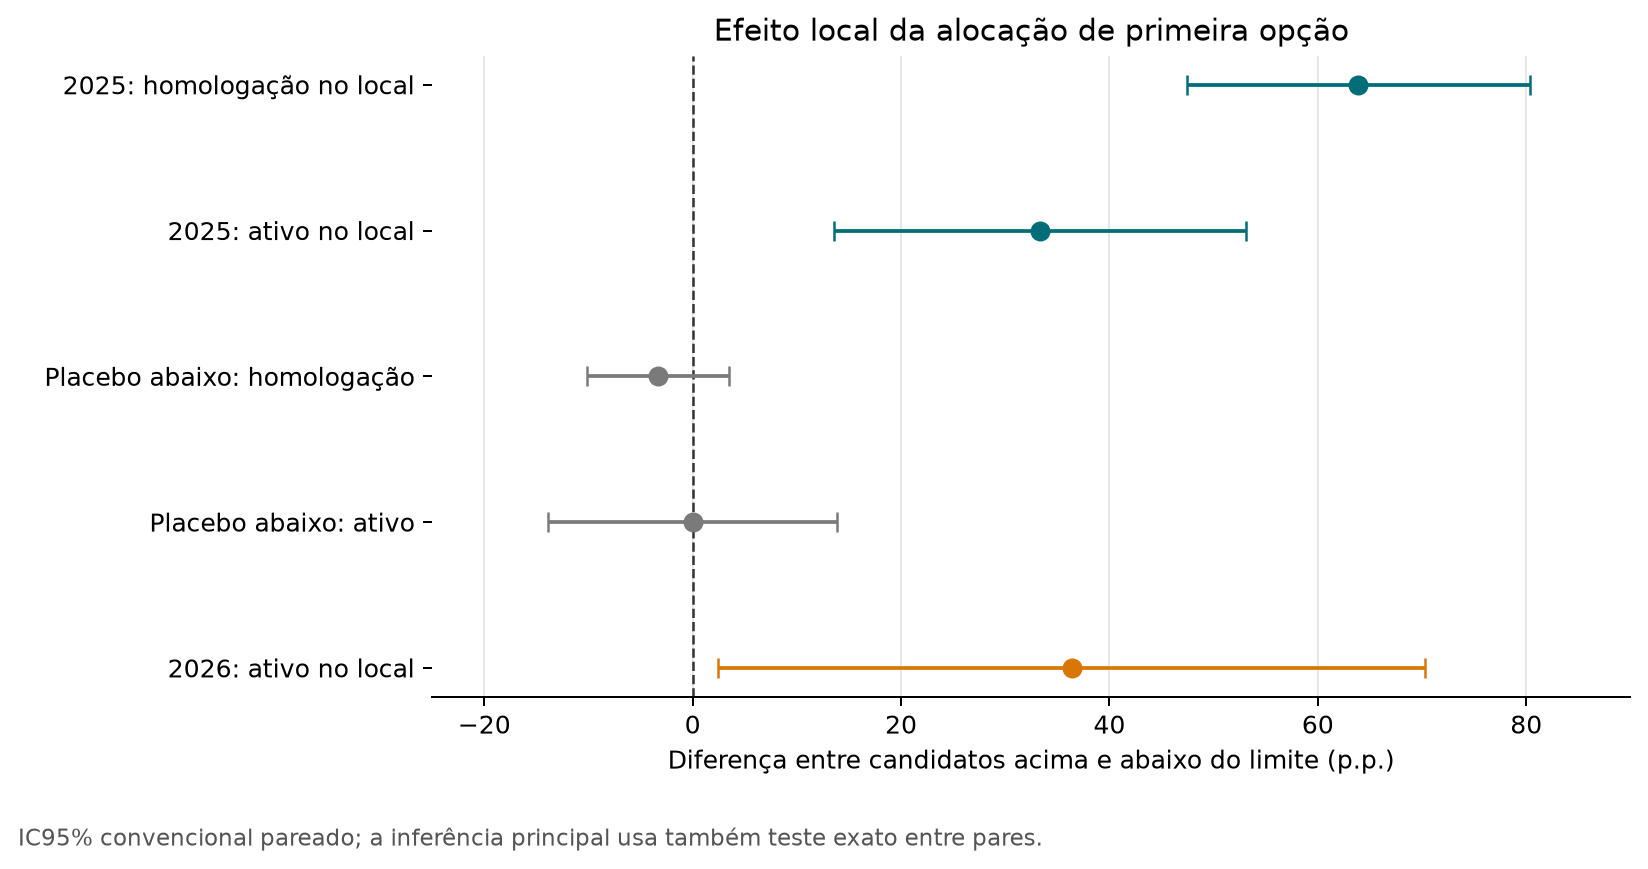
\includegraphics[width=0.94\textwidth]{output/tema_trabalho/A8_figura_01_efeitos_cutoff_escore.png}
\caption{Efeito local da alocação de primeira opção. Pontos são diferenças
pareadas entre candidatos imediatamente acima e imediatamente abaixo do limite
de seleção; barras são intervalos $t$ pareados convencionais de 95\%. A
inferência principal usa o teste exato entre pares discordantes.}
\label{fig:a8}
\end{figure}

\section{Camada descritiva: onde a atração acontece}
\label{sec:territorio}

O resultado causal diz que a alocação importa; o gradiente territorial diz onde
ela falta. A coorte contém as 1.295 células CNES--curso do quadro da primeira
chamada, em 368 municípios; o desfecho é binário por célula, alguma confirmação
ou homologação, porque confirmações em cadastro de reserva e eventos acima da
capacidade publicada impedem um denominador estável por vaga. Houve atração em
393 células, ou 30,3\% do total. A tipologia territorial, congelada antes dos
resultados a partir da REGIC 2018 e das RM/RIDE 2022, tem o interior remoto
como referência.

O modelo é linear de probabilidade, com efeitos fixos de curso e de unidade da
federação, as oito unidades de menos de cinco municípios colapsadas em
macrorregião de saúde conforme o protocolo, e erros agrupados por município. A
Tabela~\ref{tab:a4} reporta o contraste metropolitano; capital e interior
próximo a polos apresentam diferenças positivas em relação ao interior remoto,
de 32,6 e 12,1 pontos percentuais. No ajuste completo, que acrescenta IVS,
população, estoque prévio e faixa anunciada, o contraste metropolitano
permanece em 20,9 pontos percentuais, com $p$ de 0,008 e valor $q$ de 0,023
após correção FDR entre estratos; a atenuação vem quase inteiramente do
logaritmo da população, fortemente determinado pelo próprio estrato.

\begin{table}[htbp]
\centering
\small
\caption{Contraste descritivo entre células metropolitanas e interior remoto}
\label{tab:a4}
\begin{tabular}{lrr}
\toprule
Especificação ou desfecho & Diferença (p.p.) & Erro-padrão (p.p.) \\
\midrule
Modelo linear pré-especificado & 27,9 & 5,9 \\
Logit, efeito marginal médio & 25,1 & 5,2 \\
Ajuste completo & 20,9 & 7,8 \\
Apenas confirmação & 27,0 & 5,7 \\
Apenas homologação & 23,8 & 4,8 \\
Unidade município--curso & 31,6 & 5,8 \\
\bottomrule
\end{tabular}

\vspace{2pt}
\begin{minipage}{0.86\textwidth}
\footnotesize \textit{Nota:} 1.295 células e 368 municípios; erros agrupados por
município; efeitos fixos de curso e de unidade da federação. Todas as
diferenças são associativas: os estratos não são atribuídos.
\end{minipage}
\end{table}

Como o estrato capital tem 18 municípios, o protocolo exige inferência de
pequena amostra: com bootstrap selvagem agrupado, nula imposta, pesos de
Rademacher por município e 1.999 replicações, os valores $p$ são 0,0005 para
metropolitano, 0,0015 para capital e 0,0115 para interior próximo, todos
maiores que os nominais e todos abaixo de 5\%. O efeito mínimo detectável
ex-ante do contraste metropolitano era de 13,7 pontos percentuais; o ex-post,
calculado do erro-padrão realizado, é de 16,4 pontos percentuais, e é ele que
descreve a precisão do resultado.

\section{Camada associativa: o estoque cadastrado no CNES}
\label{sec:cnes}

A terceira camada pergunta se as células município--curso com atração
administrativa apresentaram trajetória distinta de oferta cadastrada. Ela mede
outro objeto, o estoque de profissionais distintos cadastrados na célula em 26
competências, de junho de 2024 a julho de 2026, e não identifica participantes
do programa, exercício efetivo nem retenção individual. A amostra confirmatória
tem 587 células em 295 municípios, restrita a dez cursos cuja ponte curso--CBO
não tem sobreposição. O modelo interage a atração realizada com cada
competência, omitindo junho de 2025, e absorve efeitos fixos de
município--curso, curso--mês e unidade da federação--mês, com erros agrupados
por município. Como atração é resultado realizado, os coeficientes são
diferenças condicionais de trajetória.

\begin{table}[htbp]
\centering
\small
\caption{Estoque cadastrado no CNES em março de 2026 relativamente a junho de 2025, amostra confirmatória}
\label{tab:a5}
\begin{tabular}{llrrr}
\toprule
Exercício & Escala & Coeficiente & EP & $p$ \\
\midrule
Atração da célula (primário) & proporcional & 0,068 & 0,018 & $<$0,001 \\
Atração da célula (sensibilidade) & nível & 0,50 & 0,23 & 0,033 \\
Placebo: município com atração, célula sem & proporcional & 0,0007 & 0,027 & 0,980 \\
Placebo: município com atração, célula sem & nível & 0,063 & 0,309 & 0,837 \\
Transbordo: vizinho da região com atração & proporcional & $-$0,011 & 0,032 & 0,741 \\
Oferta líquida por região--curso & proporcional & 0,050 & 0,018 & 0,006 \\
\quad só as que agregam $>$1 município & proporcional & 0,044 & 0,073 & 0,547 \\
\bottomrule
\end{tabular}

\vspace{2pt}
\begin{minipage}{0.92\textwidth}
\footnotesize \textit{Nota:} coeficiente do mês de março de 2026 em estudos de
evento com efeitos fixos de célula, curso--mês e UF--mês e referência em junho de
2025. A escala proporcional é o logaritmo de um mais o estoque. Nas linhas de
placebo e de transbordo, a amostra são as 372 células sem atração; no placebo, 198
estão em municípios com atração em alguma célula e 174 em municípios sem nenhuma;
no transbordo, 70 têm outro município do quadro na mesma região de saúde com
atração no mesmo curso. A oferta líquida soma o estoque por região--curso sobre
os municípios do quadro, com erros agrupados por região; das 449 região--curso,
385 contêm um único município do quadro, e nelas o agregado regional é a
própria célula, de modo que só as 64 restantes distinguem oferta líquida de
oferta da célula. Erros-padrão e valores
$p$ das linhas de placebo, transbordo e oferta líquida usam graus de liberdade
que contam os efeitos fixos absorvidos. Leitura associativa.
\end{minipage}
\end{table}

O desfecho é reportado em escala proporcional porque o nível soma profissionais
de municípios cujos estoques diferem em ordens de grandeza, e um curso de
estoque grande domina o resultado por construção. O teste conjunto dos
coeficientes anteriores à referência não rejeita zero, com $F$ de 0,63 e $p$ de
0,813. Em março de 2026, a diferença associada à atração é de 0,068 log-ponto
por célula, com erro-padrão de 0,018 e $p$ inferior a 0,001, o que corresponde
a cerca de 7\% de estoque. Na família dos 25 coeficientes de evento, o valor
$q$ de Benjamini--Hochberg desse coeficiente é 0,0034. A mesma quantidade em
nível é 0,50 profissional por célula, com erro-padrão de 0,23 e $p$ de 0,033,
mas é frágil: excluindo o curso de radiologia cai para 0,20, com $p$ de 0,366,
e ao restringir aos oito cursos cuja correspondência com o CBO é estritamente
unívoca cai para 0,12, com $p$ de 0,608; contra a média dos doze meses
anteriores é 0,41 com $p$ de 0,174; e, na família de 25 coeficientes, seu valor
$q$ é 0,364. A escala proporcional sobrevive aos mesmos exercícios, com 0,059
sem o curso de radiologia e 0,057 nos oito cursos estritos.

Três ameaças foram testadas sob protocolo escrito antes da execução
(Tabela~\ref{tab:a5}). \emph{Placebo}: entre as células sem atração, estar em
um município que atraiu em alguma outra célula não muda o estoque, com 0,063 em
nível e 0,0007 na escala proporcional; o padrão principal é da célula, não do
município. \emph{Pré-tendência por curso}: o teste conjunto pré rejeita a 5\%
nos cursos 2 e 16 na escala proporcional; excluindo-os, como a regra fixada de
antemão manda, o coeficiente de março de 2026 é 0,081, com $p$ de 0,0007, sobre
488 células. Corrigida a multiplicidade dos dez testes por curso pelo mesmo
procedimento usado nas demais famílias, só o curso 16 mantém $q$ abaixo de
0,05 na escala proporcional, com 0,0036, enquanto o curso 2 vai a 0,190; o
curso 16 é justamente aquele cujo teste conjunto tem posto de covariância
incompleto. \emph{Deslocamento}: células sem atração expostas a outro
município da mesma região de saúde com atração no mesmo curso não perdem
estoque, e a soma do estoque por região--curso sobe 0,050 log-ponto com
$p$ de 0,006 em 173 regiões. Esse segundo teste, porém, não sustenta
conclusão sobre realocação: das 449 região--curso, 385 contêm um único
município do quadro, e nelas o agregado regional é a própria célula; restrito
às 64 que de fato agregam mais de um município, o coeficiente é 0,044, com $p$
de 0,547. Deslocamento dentro da região permanece não testado, e não refutado.
O limite adicional é declarado: o painel contém apenas os 368 municípios do
quadro, de modo que ``vizinho'' é vizinho dentro do quadro.

Nada nesta seção confirma ou reforça o resultado causal da
Seção~\ref{sec:causal}: são objetos, unidades e estatutos de identificação
distintos.

\section{Rotas avaliadas e descartadas}
\label{sec:rotas}

\textbf{Regressão descontínua do adicional de bolsa pelo IVS.} A faixa de bolsa
anunciada e o Índice de Vulnerabilidade Social (IVS) são ligados por regra
administrativa. Aplicando a taxonomia externa ao IVS público, porém, 191 dos
368 municípios são reproduzidos e 177 divergem, ou 48,1\% do total; sem regra
reproduzível não há primeiro estágio, e nenhum efeito da bolsa foi estimado.

\textbf{Tripla diferença entre vaga imediata e cadastro de reserva.} No grão
município--curso e na amostra que identificaria o desenho
\citep{olden2022}, com 319 células em 93 municípios, a modalidade imediata não
prediz a alocação confirmada: a diferença ajustada é de 2,79 pontos
percentuais, com erro-padrão de 6,89 pontos percentuais e $p$ de 0,6871. O
portão de relevância não foi aprovado e a rota foi encerrada como comparação
ajustada.

Os dois descartes são anteriores ao desenho adotado e estão registrados para
que o leitor veja o conjunto de desenhos considerados.

\section{Conclusão, alcance e limites}
\label{sec:conclusao}

Sob a hipótese de comparabilidade local entre candidatos separados por um
ponto, ganhar marginalmente a vaga de primeira opção aumentou a homologação no
mesmo curso--CNES em 63,9 pontos percentuais e a presença ativa posterior
naquele mesmo curso--CNES em 33,3 pontos percentuais. O efeito aparece nas
duas chamadas de 2025, não reaparece onde a alocação não muda, é estável em
janelas de gap e exclusões sucessivas e tem direção semelhante em 2026. Em
políticas de base territorial, o desenho da alocação é parte do instrumento
\citep{kline2014}: quantas vagas abrir por célula e como tratar chamadas
subsequentes afeta onde o especialista de fato aparece.

O gradiente territorial mostra que a atração realizada é sistematicamente menor
no interior remoto, e a evidência do CNES é compatível com uma diferença
proporcional modesta de oferta cadastrada nas células com atração, robusta a
multiplicidade e a placebo municipal. O deslocamento dentro da região não foi
refutado: o teste agregado disponível não separa expansão líquida de
realocação, porque quase toda região--curso do quadro contém um único
município. Essas duas camadas são descritiva e associativa, e assim devem ser
lidas.

O desenho causal \textbf{não} identifica o efeito da bolsa nem do adicional
associado ao IVS, o efeito do programa sobre o estoque municipal, o efeito
sobre a decisão de se inscrever, retenção contínua ou duração até a saída,
produção assistencial, filas ou desfechos de saúde. Suas limitações são a
pontuação discreta com um ponto de massa de cada lado, a amostra de 36 pares, a
ligação por nome normalizado, o protocolo retrospectivo e o desfecho de
presença medido como retrato em uma data. A avaliação do adicional de bolsa
exige a regra administrativa que o IVS público não reproduz; os desfechos
assistenciais exigem portões próprios de dados. Ambos permanecem fora do
escopo.

\begin{thebibliography}{99}

\bibitem[Agarwal(2015)]{agarwal2015}
Agarwal, N. (2015). An Empirical Model of the Medical Match.
\textit{American Economic Review}, 105(7), 1939--1978.

\bibitem[Bärnighausen e Bloom(2009)]{barnighausen2009}
Bärnighausen, T.; Bloom, D. E. (2009). Financial Incentives for Return of
Service in Underserved Areas: A Systematic Review.
\textit{BMC Health Services Research}, 9, 86.

\bibitem[Carrillo e Feres(2019)]{carrillo2019}
Carrillo, P.; Feres, P. (2019). Provider Supply, Utilization, and Infant
Health: Evidence from a Physician Distribution Policy.
\textit{American Economic Journal: Economic Policy}, 11(3), 156--196.

\bibitem[Costa et al.(2024)]{costa2024}
Costa, F.; Nunes, L.; Sanches, F. M. (2024). How to Attract Physicians to
Underserved Areas? Policy Recommendations from a Structural Model.
\textit{The Review of Economics and Statistics}, 106(1), 36--52.

\bibitem[Fontes et al.(2018)]{fontes2018}
Fontes, L. F. C.; Conceição, O. C.; Jacinto, P. A. (2018). Evaluating the
Impact of Physicians' Provision on Primary Healthcare: Evidence from Brazil's
More Doctors Program. \textit{Health Economics}, 27(8), 1284--1299.

\bibitem[Gravelle et al.(2018)]{gravelle2018}
Gravelle, H.; Scott, A.; Yong, J.; McGrail, M. (2018). Do Rural Incentives
Payments Affect Entries and Exits of General Practitioners?
\textit{Social Science \& Medicine}, 216, 88--96.

\bibitem[Kline e Moretti(2014)]{kline2014}
Kline, P.; Moretti, E. (2014). People, Places, and Public Policy: Some Simple
Analytics of Local Economic Development Programs.
\textit{Annual Review of Economics}, 6(1), 629--662.

\bibitem[Olden e Møen(2022)]{olden2022}
Olden, A.; Møen, J. (2022). The Triple Difference Estimator.
\textit{The Econometrics Journal}, 25(3), 606--622.

\bibitem[Roth(1984)]{roth1984}
Roth, A. E. (1984). The Evolution of the Labor Market for Medical Interns and
Residents: A Case Study in Game Theory.
\textit{Journal of Political Economy}, 92(6), 991--1016.

\bibitem[Sivey et al.(2012)]{sivey2012}
Sivey, P.; Scott, A.; Witt, J.; Joyce, C.; Humphreys, J. (2012). Junior
Doctors' Preferences for Specialty Choice.
\textit{Journal of Health Economics}, 31(6), 813--826.

\bibitem[Sliwa Ruiz et al.(2024)]{sliwa2024}
Sliwa Ruiz, J.; Becker, S. O.; Hone, T.; Rocha, R. (2024). The Supply of
Primary Care Physicians and Population Health: Evidence from the Sudden
Departure of Cuban Doctors in Brazil.
\textit{Journal of Health Economics}, 93, 102833.

\end{thebibliography}

\end{document}
